\documentclass{bioinfo}
\copyrightyear{2016} \pubyear{2016}

\access{Advance Access Publication Date: Day Month Year}
\appnotes{Original Paper}
\newcommand{\boldm}[1] {\mathversion{bold}#1\mathversion{normal}}

\newcommand{\ddurl}{\href{http://www.data2dynamics.org/}{http://www.data2dynamics.org/}}

\begin{document}
\firstpage{1}

\subtitle{Systems Biology}

\title[$L_1$ regularization to detect differences between cell types]{{\boldm $L_1$} regularization facilitates detection of cell type specific parameters in dynamical systems}
\author[Steiert \textit{et~al}.]{Bernhard Steiert\,$^{\text{\sfb 1,}*}$, Jens Timmer\,$^{\text{\sfb 1,2}}$ and Clemens Kreutz\,$^{\text{\sfb 1}}$}
\address{$^{\text{\sf 1}}$Institute of Physics, University of Freiburg, Germany and \\
$^{\text{\sf 2}}$BIOSS Centre for Biological Signalling Studies, University of Freiburg, Germany.}

\corresp{$^\ast$To whom correspondence should be addressed.}

\history{Received on XXXXX; revised on XXXXX; accepted on XXXXX}

\editor{Associate Editor: XXXXXXX}
% This abstract is more or less a placeholder and needs to be rewritten.
\abstract{\textbf{Motivation:}
A major goal of drug development is to selectively target certain cell types.
Cellular decisions influenced by drugs are often dependent on the dynamic processing of information.
Selective responses can only be achieved by differences between the investigated cell types at levels of receptor, signaling, gene regulation, or further downstream.
Therefore, a systematic approach to detect and quantify cell type specific parameters in dynamical systems becomes necessary.\\
\textbf{Results:}
Here, we demonstrate that a combination of non-linear modeling with $L_1$ regularization is capable of detecting cell-type specific parameters.
To adapt the least-squares numerical optimization routine to $L_1$ regularization, sub-gradient strategies as well as truncation of proposed optimization steps were implemented.
Likelihood-ratio test is used to determine the optimal penalization strength resulting in a sparse solution in terms of a minimal number of cell-type specific parameters that is in agreement with the data.
The uniqueness of the solution was investigated using the profile likelihood.
By applying our implementation to a realistic \emph{in silico} dynamical model of the \emph{DREAM6} challenge we were able to recover 74\% of the differences with 20\% false positives.
Within the subset of detected differences, YY\% were in agreement with their true value.
Furthermore, we found that the results could be improved by manual inspection using the profile likelihood.\\
\textbf{Conclusion:}
The approach constitutes a general method to infer an overarching model with a minimum number of individual parameters for the particular models.
Analyzing differences between cell types enables discovering differential sensitivity to selectively target a desired cell type while leaving other cell types unaffected.
Thus, the presented methodology may facilitate directed drug design and development.\\
\textbf{Availability:} The algorithm is implemented within the freely available, open-source modeling environment Data2Dynamics \cite{Raue2015} based on MATLAB. Source code for all examples is provided online at \ddurl. [Please note: during the review process, the source code is available at \href{http://www.fdmold.uni-freiburg.de/~steiert/eccb/}{http://www.fdmold.uni-freiburg.de/\textasciitilde steiert/eccb/} with username `L1regularization' and password `ODEmodeling'. After acceptance, code and documentation will be incorporated into the official Data2Dynamics website \ddurl.]\\
\textbf{Contact:} \href{bernhard.steiert@fdm.uni-freiburg.de}{bernhard.steiert@fdm.uni-freiburg.de}
% \textbf{Supplementary information:} Supplementary data are available at \textit{Bioinformatics} online.
}

\maketitle

\section{Introduction}
The progress in the development of experimental assays like the establishment of high-throughput measurement techniques raised new demands on statistical methodology. 
Many scientific questions in the field of Bioinformatics and Systems Biology nowadays requires large models with hundreds or even thousands of parameters or variables. 
Therefore, a major issue in many applications is feature selection, i.e. determination of informative parameters or variables, which are required to explain experimental observations, for identification of differential expression and/or for making reliable predictions. 

In many cases, feature selection is equivalent to model discrimination \citep{Box67} since a set of features corresponds to a specific model with corresponding set of parameters. 
In \emph{multiple linear regression}, as an example, feature selection corresponds to choosing appropriate prediction variables used to fit an experimentally observed response variable. 
The traditional approach for choosing a suitable level of detail and the respective optimal set of features is iteratively testing many models \citep{Thompson1978}, 
i.e.~different combinations of features e.g.~by \emph{forward-} or \emph{backward selection} or combinations thereof \citep{Hocking1967, Efroymson60}. 
However, if the number of potential predictors is are large, the number of possible combinations increase dramatically as shown in Figure~1\vphantom{\ref{fig:01}}, rendering such iterative procedures as infeasible. 

Regularization techniques have been suggested as an alternative approach for selecting features and estimating the parameters in a single step. 
The idea is to estimate the parameters by optimization of an appropriate objective function, e.g.~by maximizing the \emph{likelihood}. 
If then in addition the impact of individual features is penalized, the optimal solution becomes sparse and the level of sparsity can be controlled by the strength of penalization. 
It has been shown that such penalties are equivalent to utilization of prior knowledge supplemental to the information provided by the data. 

The additional information provided by penalties reduces the variance of the estimated parameters but at the same time introduce a bias. This effect has been termed as \emph{shrinkage}. 
If the regularizing penalties are chosen appropriately, e.g. if the \emph{$L_0$}- or \emph{$L_1$-norm} are applied, a second effect occurs which can be utilized for feature selection. 
Because the $L_0$- and $L_1$-norm penalize parameters unequal to zero, only parameters remain in the model, which are mandatory for explaining the data. 
Since the penalized likelihood is discontinuous for $L_0$ regularization, $L_1$-penalties are usually preferred.

The concept of using the $L_1$-norm for data analysis and calibrating a model has been applied in several fields like for deconvolution of wavelets \citep{Taylor1979}, 
reconstruction of sparse spike trains of Fourier components \citep{Levy1981}, recovering acoustic impedance of seismograms \citep{Oldenburg1983} 
as well as for \emph{compressed sensing} \citep{Candes2008,Cheng2015} and clinical prediction models \citep{Hothorn2006}. 
Additionally, it has been used to establish statistical methods which are robust against violation of distributional assumptions about measurement errors \citep{Claerbout73, Barrodale1973}. Moreover, $L_1$ penalties have been applied to incorporate \emph{Laplacian priors} \citep{xx}. 
%
Despite this variety of applications, the usability for feature selection and a comprehensive statistical interpretation was not established until introduction of the 
\emph{LASSO (least absolute shrinkage and selection operator)}. 
This prominent approach for linear models was published in \cite{Tibshirani94} when the first affordable high-throughput techniques were available and the necessity of new approaches for analyzing high-throughput data became inevitable.

The standard LASSO has been generalized or adapted for other applications in several directions. 
Feature selection via LASSO was discussed for the regression case in more detail in \cite{tibshirani96}, for Cox-regression in \cite{Tibshirani1997}, and for clustering e.g.~in \cite{Witten2010}
The \emph{elastic net} has been introduced as a combination of $L_1$ and $L_2$ regularization \citep{Zou05}. 
The so-called  \emph{group-LASSO} has been established to select between predefined groups of features \citep{Yuan2006}, \emph{fused LASSO} accounts for additional constraints of pairs of parameters \citep{Tibshirani2005}, and  \emph{generalized LASSO} has been developed to regularize arbitrary prespecified parameter linear combinations \citep{Tibshirani2011}.
% Hier ist der Uebergang noch nicht smooth

Mechanistic  \emph{ordinary differential equation (ODE)} models are applied in Systems Biology for describing and understanding cellular signal transduction pathways or gene regulatory networks. 
For such ODE models, the feature selection issue occurs, if several cell types are considered. 
Since each cell type has different concentrations of intracellular compounds and diverse structure, each parameter of a reaction network could potentially be different. 
We suggest $L_1$-regularization in this setting to predict parameters differences between cell-types.
The components of mechanistic models have counterparts in the biological pathway of interest. 
Therefore, the models usually contain a large number of state variables representing molecular compounds and many parameters for the individual biochemical interactions. 
Therefore, the models are large and the effect of the parameters on the dynamics is typically strongly nonlinear. 
For estimating parameters in such ODE models, only a small subset of optimization routines in combination with appropriate strategies for calculating derivatives of the objective function, dealing with non-identifiability, handling of local minima etc. are applicable \citep{Raue2013}. 
We therefore augment an existing and well-tested implementation for parameter estimation for such systems \citep{Raue2015} to perform feature selection based on $L_1$-regularization. 
For this purpose, trust-region optimization \citep{Coleman96} was combined with a subgradient strategy as presented in \citep{Schmidt09} to enable efficient optimization in the presence of $L_1$-penalties. % Schon so detailliert hier?

Since shrinkage, i.e. decreasing the variance by introducing a bias is not intended for mechanistic models, we only use $L_1$-regularization for feature selection, i.e. determining the cell-type specific parameters, and then use these additional features to estimate the magnitude of the parameters in an unbiased manner. 
A suitable strategy is presented for choosing the regularization strength in this setting. 
The applicability is demonstrated using a benchmark model from the \emph{DREAM (Dialogue for Reverse Engineering Assessment and Methods)} parameter estimation challenge \citep{Steiert12}. 
The presented approach constitutes a suitable methodology for predicting cell-type specific parameters.
These could be used to predict cell-type specific sensitivities for drugs, which is a prominent challenge in cancer research.

\begin{figure}[!tpb]%figure1
\centerline{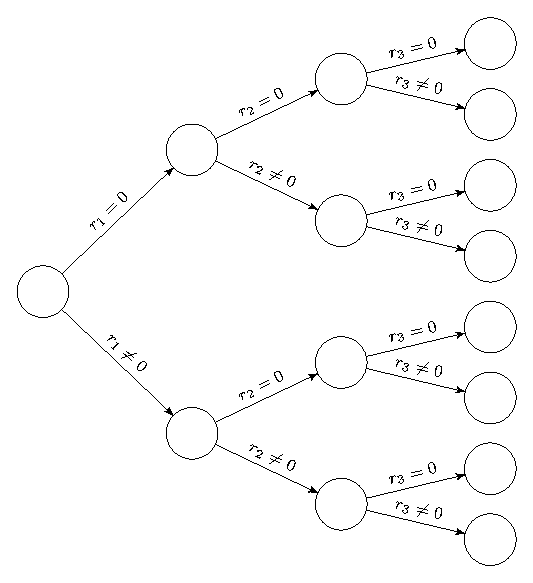
\includegraphics[width=.35\textwidth]{Figures/tree.eps}}
\caption{Na\"{\i}ve approach. Starting from the left, each log fold-change $r_i$ of parameter $p_i$ between cell types has to be chosen either cell type-independent ($r_i=0$) or -specific ($r_i\neq 0$). Hence, the number of model candidates with grows exponentially with the number of parameters.}\label{fig:01}
\end{figure}

\section{Problem statement}

Given a model $\mathcal M$ describing the kinetics of reaction network components $x_i$ with $i \in [1,\dots,m]$ by a system of ordinary differential equations (ODE)
\begin{equation}
\dot x(t) = f(x(t),u(t,p_u),p_x)\label{eq:ode}
\end{equation}
with solutions $x(t)$ representing concentrations of molecular compounds, for external inputes $u(t)$.
States $x$ are mapped to experimental data $y$ using an observation function $g$, yielding
\begin{equation}
y(t) = g(x(t),p_y)+\epsilon(t,\sigma) \:.\label{eq:obs}
\end{equation}
The error $\epsilon \sim \mathcal N(0,\sigma)$ is assumed to be normally distributed in the following.
Initial concentrations $p_0$, as well as parameters $p_x$ of the ODE, $p_u$ of the input, $p_y$ of the observation function, $\sigma$ of the error model, are subsumed in the parameter vector
\begin{equation}
p = [p_0, p_x, p_u, p_y, \sigma] \:.\label{eq:par}
\end{equation}
Therefore, the expressions (Eq~\ref{eq:ode}-\ref{eq:par}) fully specify $\mathcal M$.
To ensure positive values and improve numerics, all parameters are log-transformed.\\
Now given two cell types, each with data that can be fitted by a common ODE structure (Eq.~\ref{eq:ode}) but with differing results in their parameters $p$, i.e. $p_1 \neq p_2$.
Discovering which of the components in $p_1$ and $p_2$ are cell type-specific is the main topic of this manuscript.
A na\"{\i}ve approach would be to simply test all possibilities for cell type-specific parameters.
However, as depicted in Figure~1\vphantom{\ref{fig:01}} the number of model candidates grows exponentially with the number of parameters, rendering such an approach as infeasible.

\subsection{Unbiased parameter estimation}

To estimate parameters $p$ for $n$ data points ${y_i}$, given the corresponding observation function observation $g(t_i,p)$ which is dependent on the ODE solution, the negative two-fold log likelihood
\begin{equation}
-2\log \mathcal L(p) = \sum_{i=1}^n \frac{(y_i-g(t_i,p))^2}{\sigma_i^2} =: \chi^2\label{eq:lik}
\end{equation}
is optimized, resulting in the maximum likelihood estimate
\begin{equation}
% \hat p = \text{arg}\min \left[ -2\log \mathcal L(p) \right] \:.
\hat p = \text{arg}\min \left[ \chi^2(p) \right] \:.
\end{equation}
Multi-start deterministic local optimization is an established approach to ensure that $\hat p$ is in fact the global optimum, see \cite{Raue2013}.

\subsection{Regularization}
Regularization constitutes a prominent method to incorporate prior knowledge or to improve numerics of parameter estimation.
Here, we pursue a different strategy:
regularization is used to assess the fold-change $\tilde r_i$ of parameters between cell type 1 (ct1) and cell type 2 (ct2), i.e. $p_{i,\text{ct1}} = \tilde r_i \cdot p_{i,\text{ct2}}$.
Therefore, the constrained likelihood
\begin{equation}
\chi^2_{L_k}(p,r) = \chi^2(p) + \lambda \sum_i ||\log \tilde r_i||_k\label{eq:likreg}%\vspace*{-4pt}
\end{equation}
is implemented consisting of the likelihood (Eq.~\ref{eq:lik}) and a $L_k$ regularization term weighted by $\lambda$.
In the following, we substitute $r_i := \log \tilde r_i$.
The regularization term corresponds to a prior in a Bayesian framework:
for $k=0$ the $L_0$ prior is a delta distribution, for $k=1$ the $L_1$ prior is Laplacian function, and for $k=2$ the $L_2$ prior is a Gaussian function.
Using the definition
\begin{equation}
||r_i||_k := {\left( \sum_{j=1}^n |r_{ij}|^k \right)}^{1/k}\label{eq:norm}%\vspace*{-4pt}
\end{equation}
of a $k$-norm, we derive properties of $L_k$ for ranges of $k\in \mathbb R$.
$L_0$ would be ideal for our task due to its' direct penalization of the number of $r_i \neq 0$.
However, $L_0$ is not recommended because the associated optimization problem is known to be NP-hard, i.e. the exact solution cannot be obtained within polynomial computation time.
In general, for $k<1$, the $L_k$ metric is non-convex which severely hampers parameter estimation.
On the positive side, $k\leq1$ and especially both $L_0$ and $L_1$ induce sparsity with the results usually being similar.
In contrast, the $L_k$ metric for $k>1$ does not lead to sparse results.
$L_2$, which is simply the well-known least squares, can be handled extremely efficient but is not able to produce sparse results without introducing heuristics.
In that sense, the $L_1$ metric is unique because it is the only one that combines both features, convexity and sparsity.
Therefore, $L_1$ is the natural choice for feature selection and is used following.
% Due to local optima, the MLE (Eq.~\ref{eq:lik}) is obtained for individual cell types.
Figure~2\vphantom{\ref{fig:02}} demonstrates how sparsity is induced by the $L_1$ norm.
In the upper row, a quadratic ($L_2$) contribution is shown by the solid black lines, representing for an arbitrary linear model.
The $L_1$ contribution is shown by the dashed blue lines.
With increasing $\lambda$ from panels left to right, the influence of the $L_1$ term is increased.
The lower row shows the constrained likelihood (Eq.~\ref{eq:likreg}), i.e. the sum of the two lines in the corresponding upper panels.
For $\lambda=0.5$, the minimum is biased towards zero (middle panel) in contrast to the unregularized minimum (left panel) but different from zero.
In contrast, the minimum is exactly at zero for $\lambda=2$ (right panel).

\begin{figure}[!tpb]%figure1
\centerline{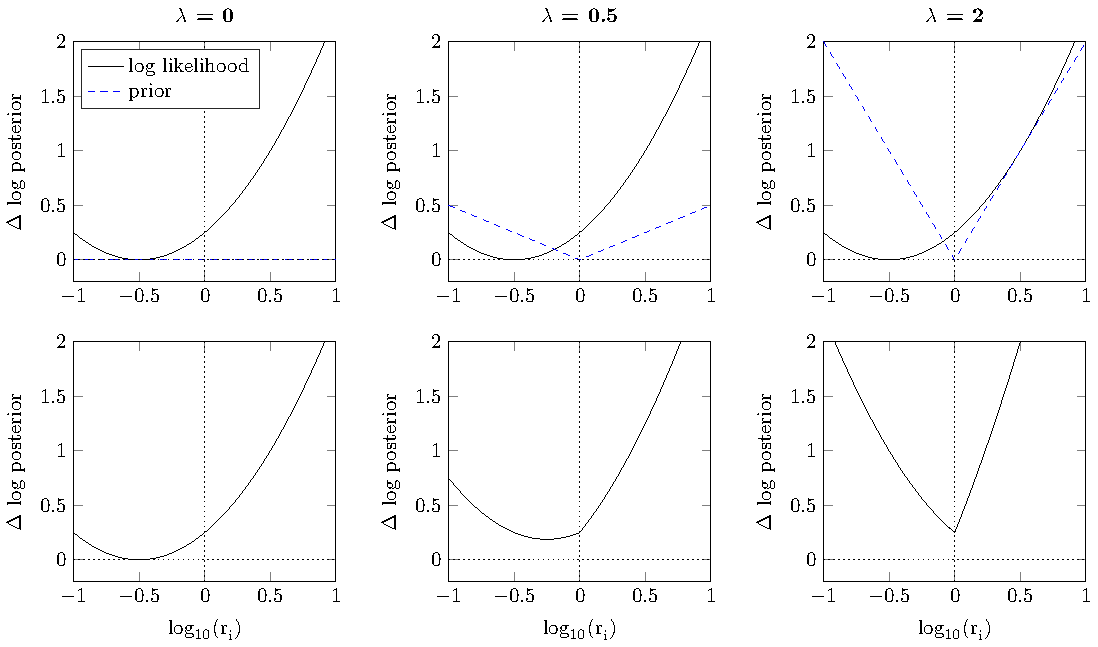
\includegraphics[width=235pt]{Figures/l1_cartoon_priorstrength.pdf}}
\caption{Sparsity and bias introduced by $L_1$ regularization. Regularization weight $\lambda$ increases from panels left to right. In the upper row, the contributions from a least-squares term ($L_2$) and an $L_1$ regularization term are shown. Their sum is plotted in the lower row. For $\lambda=0.5$, a bias is introduced shifting the minimum towards zero (middle column). When $\lambda$ is increased to 2 (left column), the minimum is exactly at zero, i.e. sparsity is induced.}\label{fig:02}
\end{figure}

\subsection{Regularized parameter estimation}
Optimization in context of partially observed stiff non-linear coupled ODE is challenging.
However, methods have been developed to efficiently compute solutions to this problem.
To augment the existing implementations with $L_1$ regularization, i.e. to minimize the constraint likelihood
\begin{equation}
	\chi2_{L_1}(p,r,\lambda) = \chi^2(p) + \lambda \sum_i |r_i|
\end{equation}
the following considerations were taken.
Efficient optimization routines like Gauss-Newton or Levenberg-Marquardt exploit the quadratic form in (Eq.~\ref{eq:lik}).
For example, the implementation of a trust-region method \textit{lsqnonlin} in Matlab expects residuals
\begin{equation}
	\text{res}_j = \frac{y_j-g(t_j,p)}{\sigma_j}
\end{equation}
for data points $y_j$ as input and implicitly calculates the value of the objective function by summation over squares of all residuals.
To realize optimization of the constrained likelihood (Eq.~\ref{eq:likreg}),
\begin{equation}
	\text{res}_i = \sqrt{\frac{|r_i|}{1/\lambda}}
\end{equation}
is appended to the residuals vector for each fold-change $r_i$.
The associated sensitivities to the regularization residuals $\text{res}_i$ are calculated as
\begin{equation}
	\text{sres}_{ii} = \frac{\partial \text{res}_i}{\partial r_i} = \frac{\text{sgn}(r_i)}{\frac{2}{\lambda}\sqrt{\frac{|r_i|}{1/\lambda}}} \:.\label{eq:sres}
\end{equation}
Therefore, the gradient components
\begin{equation}
	g_i = 2 \: \text{res}_i \cdot \text{sres}_{ii} = \pm \lambda
\end{equation}
match the expected theoretical value, which is the constant slope $\pm \lambda$ induced by the $L_1$ term.
For $r_i = 0$, Eq.~\ref{eq:sres} is not defined.
In this case, the convergence criterion
\begin{equation}
	\begin{cases}
	\nabla_i \chi^2(\hat r_i) + \lambda \text{ sign}(\hat r_i) = 0, \:\:& |\hat r_i| > 0\\
	|\nabla_i \chi^2(\hat r_i)| \le \lambda, \:\:&\hat r_i = 0 \:.
	\end{cases}
	\label{eq:convcrit}
\end{equation}
is implemented by setting
\begin{equation}
	\begin{cases}
	\text{sres}_{ii}=0&|\nabla_i \chi^2(r_i)| > \lambda\\
	\text{sres}_{ij}=0\:\:\forall j, \:\:&|\nabla_i \chi^2(r_i)| \le \lambda \:.
	\end{cases}
	\label{eq:sresset}
\end{equation}
The rationale behind Eq.~\ref{eq:convcrit} is that the $L_1$ gradient either compensates the data gradient (first line), or that the $L_1$ dominates the data gradient and constrains the estimate to its center $\hat r_i=0$ (second line).
During optimization, this parameter-wise convergence criterion is checked for each candidate $r_i=0$ at every optimization step.
While the criterion is fulfilled, the derivative of each residual $j$ with respect to $r_i$ is set to zero, i.e. $\text{sres}_{ij}=0\:\:\forall j$.
Thereby, the optimizer is unable to change $r_i$ to a non-zero.
If at certain optimization step, the convergence criterion is violated, only the $i$th $L_1$ contribution to the gradient is set to zero.
This in turn enables $r_i$ that were zero to be released during optimization if there is enough evidence in the data.

The $L_1$ metric has a discontinuous derivative at zero.
In other words, the optimization routine encounters unexpected jumps of the derivatives as the sign of $r_i$ changes.
For $n$ parameters, there exist $2^n$ combinations of signs.
These hyper-quadrants are called orthants.
For an efficient optimization, proposed optimization steps that change the orthant have to be avoided.
There are several methods that cope with this problem.
They have in common that they divide a proposed optimization step into two:
first a step towards zero, then moving on.
Their major difference is the strategy how to step towards zero.
To mimic most of original behavior of trust-region based methods, we implemented the truncation of an optimization step such that the orthant is maintained.
Both convergence and truncation are depicted in Figure~3\vphantom{\ref{fig:03}}.

\begin{figure}[!tpb]%figure1
\centerline{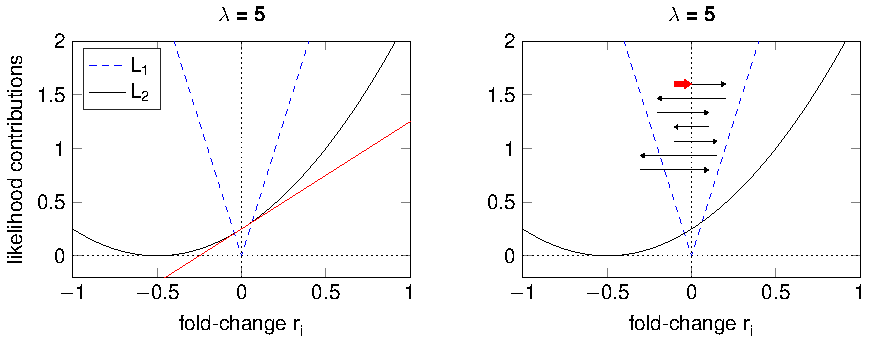
\includegraphics[width=235pt]{Figures/l1_cartoon.pdf}}
\caption{Convergence criterion and truncation. Left panel: the implementation considers a $L_1$ regularized parameter $r_i$ to be converged if the gradient contribution, i.e. slope, from the data ($L_2$ - black line) is smaller than the slope of the $L_1$ term (dashed blue line). For $r_i=0$, the algorithm compares the red line, which is the slope of the black line at this point, to the blue dashed line. Here, the slope of the $L_1$ term is larger than of the $L_2$ term, hence the corresponding entries in the sensitivity matrix are set to zero. Right panel: The black arrows give a cartoonish representation of optimization steps. To avoid jumping back and forth, i.e. numerical instability by changing the sign of $r_i$ due to discontinuously changing slope of $L_1$, an optimization step is truncated such that the sign of all $r_i$ does not change. In this case, the optimizer thereby converges in one step.}\label{fig:03}
\end{figure}

\subsection{Profile likelihood}
The \emph{profile likelihood (PL)} constitutes a method to assess confidence intervals of parameters or predictions, see \cite{Raue2009} and \cite{Kreutz2012} for an overview.
It does not require asymptotic assumptions and therefore performs well even for strongly non-linear problems.
The basic idea is to fix a certain model quantity, e.g. a parameter of interest, to a value and re-optimize all other parameters. % Formula?
This re-optimization procedure is iterated for different fixed values of the quantity of interest.
By comparing the decrease in goodness-of-fit confidence regions are calculated.

Here, we use \emph{PL} to check the parameter differences discovered by our algorithm.
Thus, the un-regularized \emph{PL} of fold-change parameter $r_i$ that is proposed using $L_1$ regularization is calculated.
If selection was successful, the \emph{PL} should not be compatible with 0.
This interpretation is equivalent to a likelihood ratio test between the null model $r_i=0$ and the alternative model $r_i \neq 0$.
% However, the results are not expected to match exactly due to parameter dependencies that prevent $r_i=0$ for the regularized problem.
Note that we did not use \emph{PL} in the first place, as the combinatorial issue shown in Figure~1\vphantom{\ref{fig:01}} is not solved by this approach.

In addition, \emph{PL} can be used to investigate the uniqueness of the solution.
A non-uniquely selected parameter could be e.g. exchanged with another parameter that was not selected as difference.
Therefore, the \emph{PL} for each $r_i$ with estimate $\hat r_i=0$ is calculated.
This is equivalent to testing a model with 1 additional parameter ($r_i$) in comparison to parsimonious model ($r_i \equiv 0$).
If inside the CI of $r_i$, another parameter that was different to $0$ is now compatible with $0$, one cannot decide on the data which one is different.

%Finally, regularized \emph{PL} of selected differences can pinpoint compensating effects.
%Compensation manifests in piecewise flat regions in \emph{PL} though the regularization alone should already induce non-zero derivatives of \emph{PL}.
%However, if a parameter change is compensated by adjusting another parameter, the regularizations can cancel out as well.
%The \emph{PL} shape is then a clear indicator for compensation.

\subsection{Regularization strength $\lambda$}
For generating model candidates, $\lambda$ is increased and the likelihood is re-optimized until mismatch between model and data is too large to reject the associated simplification.
This strategy is similar to the calculation of \emph{PL}, where a parameter of interest is fixed and the remaining parameters are re-estimated.
In both cases, likelihood-ratio statistics are employed to discover admissible regions.
For $L_1$ based feature selection, cross validation is often used to choose the final value for the regularization weight $\lambda$.
However, in nonlinear modeling, leaving data out could produce non-identifiablilites and the effect on the prediction error can be ambiguous.
Therefore, we decided to use an information theory based test criterion.
The most prominent methods are the likelihood ratio test (LRT), the Akaike information criterion (AIC), and the Bayesian information criterion (BIC).
The criteria are depicted by the vertical lines in Figure~4\vphantom{\ref{fig:04}} for an exemplary regularization path.
In certain settings these are equivalent: AIC resembles LRT for $\alpha = 15.6\%$.
With growing model size, $\alpha$ should be adjusted.
As this is not the case for AIC, we favor LRT over AIC.
BIC takes model size into account and is therefore equivalent to LRT with adjusted $\alpha$.
Because the selection criteria BIC and LRT hence comparable, we only use LRT in the following without loss of generality.
Given a scan of $\lambda$.
Then, each $r_i$ either equals zero or not, depending on $\lambda$.
In a second step the $L_1$ regularization is omitted and the unbiased maximum likelihood estimate is calculated, under the side constraint that fold-changes with $r_i=0$ are fixed to zero.
The value of the objective function for this constrained unbiased solution is denoted as $\chi^2_\lambda$.
The LRT statistics
\begin{equation}
	D_\lambda = \chi^2_\lambda - \chi^2_{\lambda=0}
\end{equation}
quantifies the discrepancy to the full model with only cell type-specific parameters.
The cut-off for determining the \emph{parsimonious model}, i.e. the model with a minimal number of differences for given $\alpha$ level which is able to fit the data is given by the $\chi^2_{m_\lambda,\alpha}$ distribution with degrees of freedom $m_\lambda=\#r_i - \#(r_i=0)_\lambda$.
Thus the \emph{parsimonious model} is given by
\begin{equation}
	\lambda^* = \arg \lceil D_\lambda < \chi^2_{m_\lambda,\alpha} \rceil \:.
\end{equation}
We use $\alpha = 0.05$ in the following.
% At the end, a good method should optimize specificity and sensitivity.
% Thus, the result should appear as far as possible to the upper-left corner of the ROC curve.

\begin{methods}
\section{Approach}
% This section needs improvement. What are the exact steps to be performed for L1 analysis?
Given an overarching model that is able to describe two cell types with parameter vectors $p_1$ and $p_2$ for cell types 1 and 2, respectively.
Eq.~\ref{eq:likreg} is used to $L_1$ penalize the fold-change parameters $r$.
Then, $\lambda$ is scanned and the number of cell type specific parameters is observed.
For choosing the optimal $\lambda$, the un-regularized Eq.~\ref{eq:lik} is optimized, under the constraint that parameters with $r_i = 0$ are shared between both cell types.
The full model with all parameters specific for each cell type is then compared by the likelihood ratio test to each of the models that were selected using $L_1$ regularization.
Finally, the most parsimonious model is defined as the smallest model that cannot be rejected by the likelihood ratio test.\\
Exemplary, we investigate uniqueness by \emph{PL}.
For giving a statistical assessment of the method it is unfeasible to perform this supervised uniqueness analysis for each iteration.
However when applied in practice results can be further improved by this manual analysis.
To mimic the manual inspection of the results, we implemented a heuristic that tests each $L_1$ parameter against zero from their order of deviation from zero.
If the likelihood did not increase by more than 1, the correction was accepted.
We show exemplarily for the application how the heuristic performs against a supervised manual inspection.
Further, plotting unobserved components for both cell types can enables validation design by discovering dynamics with a small prediction CI, which are different between the cell types.

%Text Text Text Text Text Text  Text Text Text Text Text Text Text
%Text Text Text Text Text Text Text Text.
%Figure~2\vphantom{\ref{fig:02}} shows that the above method  Text
%Text Text Text Text Text Text Text Text Text  Text Text.
%\citealp{Boffelli03} might want to know about text text text
%text\vspace*{1pt}
%
%\begin{itemize}
%\item for bulleted list, use itemize
%\item for bulleted list, use itemize
%\item for bulleted list, use itemize\vspace*{1pt}
%\end{itemize}
%
%Text Text Text Text Text Text  Text Text Text Text Text Text Text
%Text Text Text Text Text Text Text Text.
%Figure~2\vphantom{\ref{fig:02}} shows that the above method Text
%Text Text Text Text Text Text Text Text Text Text Text.
%\citealp{Boffelli03} might want to know about text text text text
%Text Text Text Text Text Text  Text Text Text Text Text Text Text
%Text Text Text Text Text Text Text Text.
%
%Text Text Text Text Text Text  Text Text Text Text Text Text Text
%Text Text  Text Text Text Text Text Text\vadjust{\newpage}.
%Figure~2\vphantom{\ref{fig:02}} shows that the above method  Text
%Text Text Text  Text Text Text Text Text Text  Text Text.
%\citealp{Boffelli03} might want to know about text text text text
%
%
%\subsection{This is subheading}
%
%Text Text Text Text Text Text Text Text Text Text Text Text Text
%Text Text  Text Text Text Text Text Text.
%Figure~2\vphantom{\ref{fig:02}} shows that the above method  Text
%Text Text Text Text Text Text Text Text Text  Text Text.
%\citealp{Boffelli03} might want to know about  text text text text
%Text Text Text Text Text Text  Text Text Text Text Text Text Text
%Text Text  Text Text Text Text Text Text.
%
%
%\subsubsection{This is subsubheading}
%
%Text Text Text  Text Text Text Text Text Text  Text Text.
%\citealp{Boffelli03} might want to know about  text text text text
%Text Text Text Text Text Text Text Text Text Text Text Text Text
%Text Text  Text Text Text Text Text Text.
%Figure~2\vphantom{\ref{fig:02}} shows that the above method  Text
%Text Text Text  Text Text Text Text Text Text  Text Text.
%\citealp{Boffelli03} might want to know about  text text text text
%
%\enlargethispage{6pt}
%
%
%Text Text Text Text Text Text  Text Text Text Text Text Text Text
%Text Text  Text Text Text Text Text Text.
%Figure~2\vphantom{\ref{fig:02}} shows that the above method  Text
%Text Text Text  Text Text Text Text Text Text  Text Text.
%\citealp{Boffelli03} might want to know about  text text text text


\end{methods}

%\begin{figure}[!tpb]%figure2
%%\centerline{\includegraphics{fig02.eps}}
%\caption{Caption, caption.}\label{fig:02}
%\end{figure}

%Text Text Text Text Text Text  Text Text Text Text Text Text Text
%Text Text  Text Text Text Text Text Text.
%Figure~2\vphantom{\ref{fig:02}} shows that the above method  Text
%Text Text Text  Text Text Text Text Text Text  Text Text.
%\citealp{Boffelli03} might want to know about  text text text text\vspace{10pt}

\section{Application}
\subsection{Model description}
In the following, we use the first model of the \emph{DREAM6 (Dialogue for Reverse Engineering Assessment and Methods)} challenge as benchmark for our approach.
The in-silico model mimics a gene-regulatory network and is based on realistic assumptions.
It was used in 2011 to evaluate the performance of experimental design strategies to optimize parameters and predictions.
The model incorporates transcription and translation dynamics of 6 genes.
Therefore, the dynamic variables represent 6 mRNAs, as well as the 6 associated proteins with known initial concentrations.
Positive and negative regulation between genes is possible.
Taken together, the model consists of 29 parameters.
13 are associated with generation and degradation of molecules:
1 protein degradation rate which is shared among all proteins; 
6 ribosomal strengths determining the production rate of mRNAs;
6 protein production strengths which define how strong mRNA presence induces protein synthesis;
The remaining 16 parameters define the interaction of genes by Hill kinetics, thus 8 $K_D$ values and 8 Hill coefficients are assumed.

DREAM6 M1 was simulated with gold-standard parameters that were made publicly available after completion of the challenge.
We now use this gold-standard as cell type 1.
When complete data is provided, i.e. all observables measured at all possible experimental conditions, all parameters are identifiable, except for one Hill coefficient which is only restricted to lower values.
Thus, we conclude that determining parameter differences between cell types is possible in principle.
Next, we assumed 1/3 of all parameters to be cell type-specific.
We therefore randomly simulated fold-changes of $[2~5~10]$ for non-Hill parameters in both directions.
For Hill coefficients, fold changes of $1/2$ and $1/4$ were assumed, under the constraint that the modified values stay inside the interval $[1~4]$.
This assumption for the range is biologically reasonable as the number of binding sites on a molecule is thereby considered.
Taken together, the number of possible models is $2^{29}>5\cdot10^8$.

In the original DREAM6 challenge, there were basically two observation types available:
(1) mRNA measurements for all mRNAs with 21 data-points each, or (2) protein measurements for 2 proteins which had to be specified, each with 41 data-points.
The observation function was the identity, i.e. the molecular compounds were observed directly without scaling or offset parameters.
The error model was consisted of an absolute term as well as a relative term with given contributions.
% If a trajectory was near zero, negative data points may occur which were then set to zero to avoid negative concentrations.
In addition to wildtype data, there was the option of performing 3 possible perturbations per each node $i$ out of 6 nodes:
\begin{enumerate}
\item knock-out ($\text{mRNA\_pro}_i=\text{Prot\_pro}_i=0$)
\item knock-down ($\text{mRNA\_deg}_i\rightarrow 5\cdot \text{mRNA\_deg}_i$)
\item over-expression ($\text{mRNA\_pro}_i \rightarrow 2\cdot \text{mRNA\_pro}_i$)
\end{enumerate}
In total, this results in 18 possible experimental conditions.
To have a reference for perturbations we decided during the original challenge to purchase all wildtype data, i.e. mRNA and protein data for all observables.
After acquiring wildtype data the remaining budget was sufficient for around 9 additional data sets, which had to be selected from $331$ possibilities.
To allow some variability in the number of experiments, we randomly (50\%) selected for each of the 18 conditions whether the conditions was included in the observation.
To mimic the partial observation which was one task of the DREAM6 challenge, we chose random whether mRNA (1/3) or proteins (2/3) were observed.
Given the latter, 2 out of 6 proteins were randomly selected.
We chose the same experimental conditions and observables for both cell types.

After implementing the fold-changes between cell types, as well as perturbations and observations we used a $L_1$ regularization for all fold-change parameters and scanned along $\lambda$ for variable selection.
For selection of $\lambda$ we used the unpenalized solution.
Thus, we could ensure an unbiased estimate of the fold-change parameters.

\begin{figure}[!tpb]%figure1
\centerline{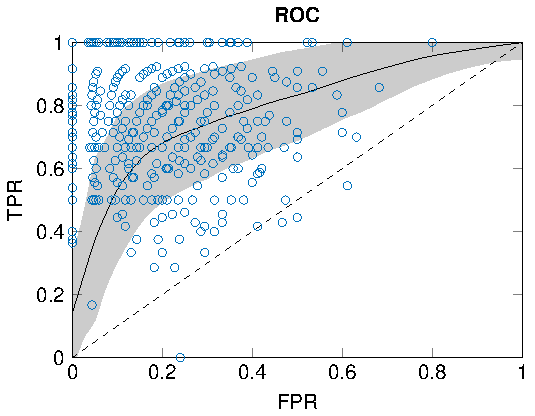
\includegraphics[width=235pt]{Figures/ROC.pdf}}
\caption{ROC curve displaying the performance of the implementation on DREAM6 M1. No experimental design was performed. $N = 500$. Black line is average ROC curve. Shading is standard deviation. Blue circles denote selected model for all iterations. Because the dots appear on average near the maximum of sensitivity and specificity (upper left corner), we consider our selection criterion as appropriate.}\label{fig:04}
\end{figure}

\subsection{Performance assessment}
The procedure of selecting fold-changes and observations was iterated $N=500$ times, yielding a random sample of $2^{29} \cdot 331 > 10^{11}$ possibilities.
The performance is summarized in Figure~4\vphantom{\ref{fig:04}}.
The black line depicts the average ROC curve, the shading gives the standard deviation over all $N=500$ iterations.
The blue dots show the selected parsimonious model selected by the likelihood-ratio test.
Usually, for a given ROC curve the selection criterion is chosen to maximize both sensitivity and specificity simultaneously, which is the point most up-left on the ROC curve.
Because the blue dots appear centered around this `kink', we consider our selection criterion appropriate.
Despite missclassification, out of the true positives XX\% were estimated closest to their true fold-change.
Thus we conclude that the unbiased estimates for fold-changes are robust against errors in classification.

We further evaluated the performance of our $L_1$ fold-change detection routine for different parameter types.
The results are summarized in Table~1\vphantom{\ref{Tab:01}}.
The protein degradation rate is shared among all proteins.
It is detected in 100\% as difference when there was a difference simulated.
On the other hand, this parameter also had the highest false positive rate with approximately 46\%.
A possible explanation is given by the fact that our method is data driven and hence differences are more likely to be detected in points of the network with more data available.
This is the case for the protein degradation rate because it influences all proteins in the network.
The individual protein production and ribosomal strengths have a false positive rate around 20\% and a true positive rate of approximately 80\%.
In contrast, the Hill regulation parameters ($K_D$ and Hill coefficient) are detected less frequently as difference.
Probably, this is due to identifiability issues as those parameters were already the most difficult ones to estimate in the original DREAM6 challenge.
The underlying reason is that the concentration range around $K_D$ has to be sampled for a reliable estimation, which cannot be ensured without proper experimental design.

% Performance for different fold-changes\\ % Wie bewertet man das am besten? Braeuchte man evtl. Unsicherheitsabschaetzungen ...
% Performance for different ratio of protein vs mRNA measurement % Ist das spannend?

\begin{table}[!t]
\processtable{Performance of algorithm on DREAM6 M1\label{Tab:01}} {\begin{tabular}{@{}llll@{}}\toprule Parameter class &
N & FPR & TPR\\\midrule
Protein degradation rate & 181 & 0.4577 & 1.0000\\
Protein production strength & 1032 & 0.2393 & 0.7965\\
Ribosomal strength & 986 & 0.1927 & 0.7982\\
$K_D$ value & 1365 & 0.1624 & 0.6989\\
Hill coefficient & 1311 & 0.1852 & 0.6461\\\hline
All & 4875 & 0.2006 & 0.7366\\\botrule
\end{tabular}}{Protein degradation rate is shared among all and hence often diagnosed as difference. Strengths are well-balanced for FPR and TPR. $K_D$ and Hill coefficients are difficult to detect because concentration range around $K_D$ has to be covered to see effect on dynamics. 500 iterations were computed. Each iteration ($L_1$ regularized scan; unregularized fits) took 28.8 min on average on an Intel Xeon E5-1620 3.60Ghz desktop computer.}
\end{table}

\subsection{Manual inspection}
In the following, we select one representative iteration out of the $N=500$ given by a minimal deviation of its ROC curve to the average ROC curve.
For the automatic model selection shown in the previous section, $\lambda$ was scanned around the selected value.
Now, we use a higher grid density for $\lambda$ to visualize the regularization path in Figure~5\vphantom{\ref{fig:05}}.
% Next, we calculate \emph{PL} for each regularized parameter to check for compensating effects.
We checked by calculating \emph{PL} of the unregularized fold-change parameters whether the results are not compatible with zero (Figure~6\vphantom{\ref{fig:06}}).
This facilitates the removal of 3 additional parameters which are all false positives.
In comparison to the automatically detected parameter differences, the result of the manual inspection decreased the FPR from XX\% to YY\% and increased the TPR from XX\% to YY\%.
Further, we checked uniqueness of the solution as shown in Figure~7\vphantom{\ref{fig:07}}.
We therefore advise manual inspection in a real world application to maximize the performance of the method.

\begin{figure}[!tpb]%figure1
\centerline{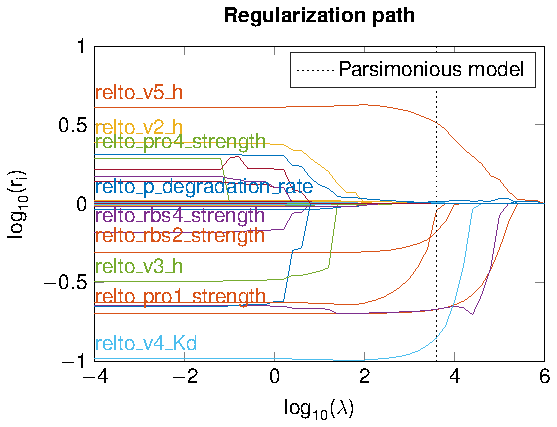
\includegraphics[width=110pt]{Figures/l1_tree.pdf}~~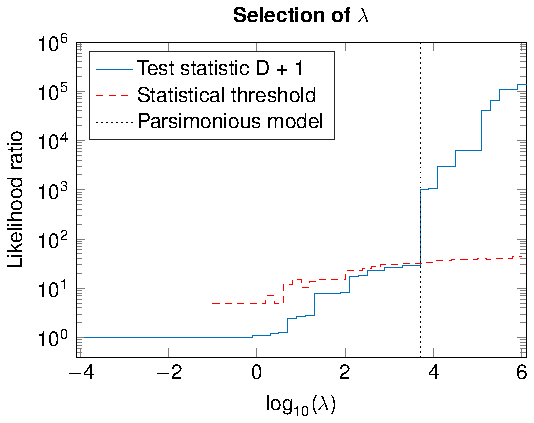
\includegraphics[width=110pt]{Figures/l1_selection.pdf}}
%\centerline{\includegraphics{fig01.eps}}
\caption{Left: Regularization path of a representative iteration. On the x-axis, the regularization weight $\lambda$ is denoted. As $\lambda$ is increased, the number fold-changes unequal to zero is reduced and the estimates are shrinked towards zero. An arbitrary subset is denoted. As expected for non-linear models, the individual paths are not necessarily monotonous. The vertical dashed lines depicts the parsimonious model. Right: Selection of $\lambda$. The likelihood-ratio test statistic D is calculated for each value of $\lambda$ (blue solid line). The value where D crosses the statistical threshold (dashed red line) marks the most parsimonious model (dashed black line).}\label{fig:05}
\end{figure}

\begin{figure}[!tpb]%figure1
\centerline{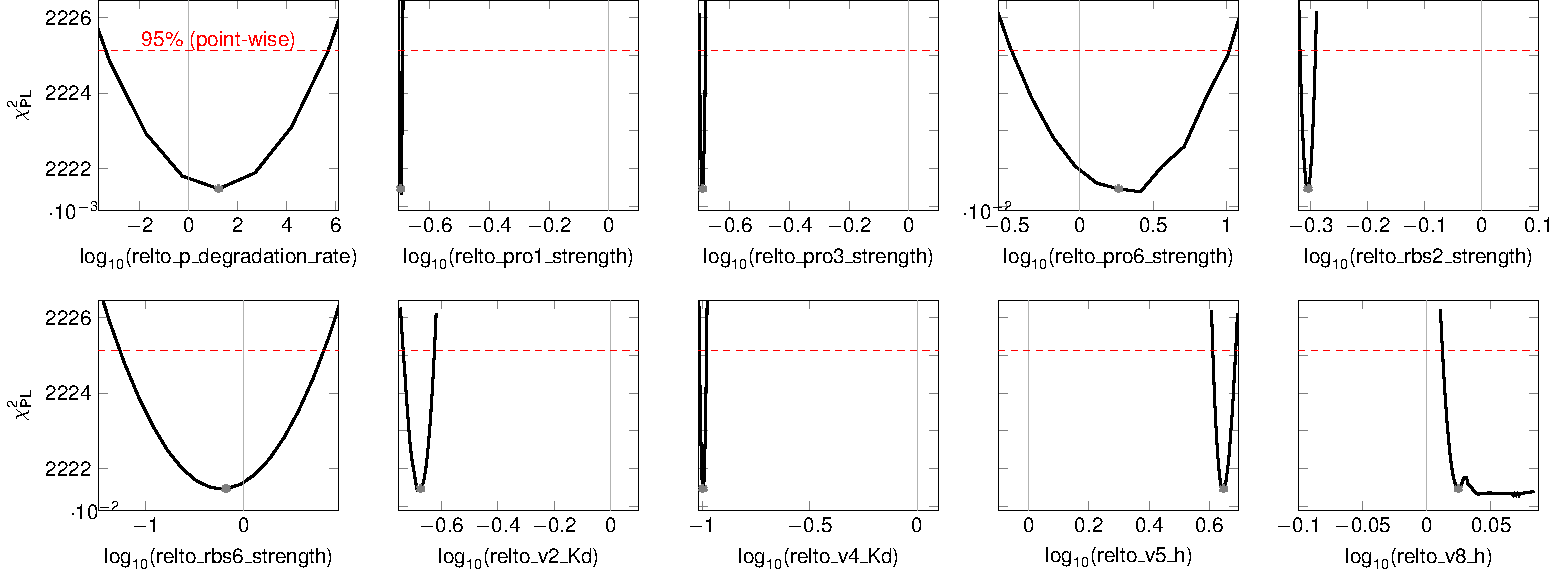
\includegraphics[width=235pt]{Figures/multi_plot.pdf}}
\caption{Determining fold-changes that are compatible with zero (gray vertical line) using \emph{PL}. Both parameters in the first column, and the one in the first row, fourth column are compatible with zero. These were actually false positives that could be transformed into true negatives by this analysis.}\label{fig:06}
\end{figure}

\begin{figure}[!tpb]%figure1
\centerline{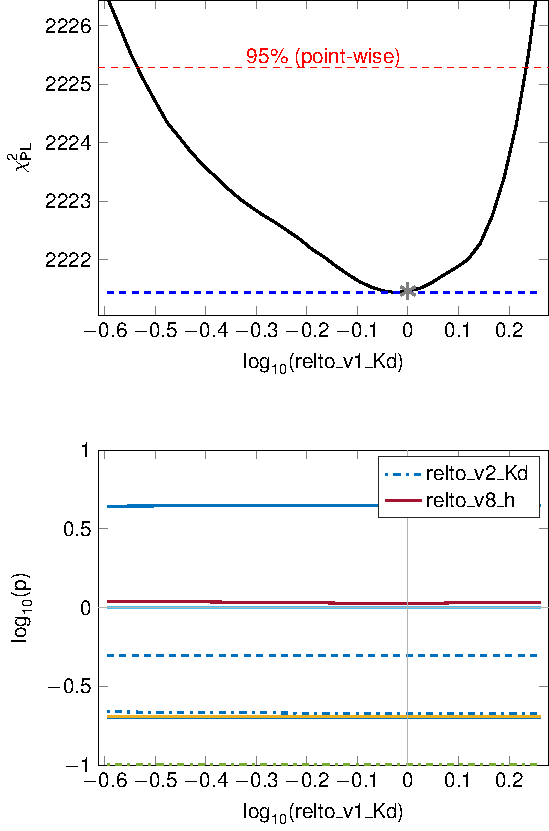
\includegraphics[width=110pt]{Figures/uniqueness_1.pdf}~~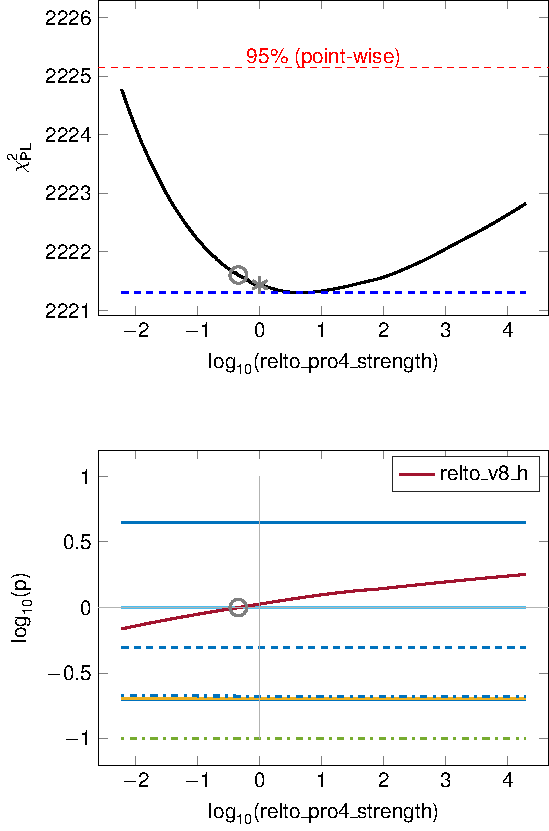
\includegraphics[width=110pt]{Figures/uniqueness.pdf}}
\caption{Uniqueness and exchangeability. To check the uniqueness of a solution we test using \emph{PL} whether ($r_i=0$ and $r_j\neq0$) gives an equivalent results as ($r_i\neq0$ and $r_j=0$) for $i\neq j$. The results of the manual inspection example are shown. On the upper row, \emph{PL} of a fold-change parameter that was estimated to zero is shown. The optimum (asterisk) is not at the minimum because the unbiased solution is computed. On the lower row, the respective values of the other $\{r_i\}$ are shown. When a parameter that was non-zero is compatible with zero, it is marked with a circle. On the left hand side the fold-change parameter of $K_{D,1}$, which is a true negative, cannot be exchanged with any other parameter. However, on the right hand side, a false negative fold-change $r_{pro4}$ could be exchanged with the false positive Hill coefficient $r_{H8}$. Thus although the solution classifies both parameters incorrectly, it pinpoints the possibility of the correct solution. Given the available data, these cannot be distinguished and experimental design would be necessary to decide which one is cell type specific, or both.}\label{fig:07}
\end{figure}


%Text Text Text Text Text Text  Text Text Text Text Text Text Text
%Text Text  Text Text Text Text Text Text.
%Figure~2\vphantom{\ref{fig:02}} shows that the above method  Text
%Text Text Text  Text Text Text Text Text Text  Text Text.
%\citealp{Boffelli03} might want to know about  text text text text
%
%
%Table~\ref{Tab:01} shows that Text Text Text Text Text  Text Text
%Text Text Text Text. Figure~2\vphantom{\ref{fig:02}} shows that
%the above method Text Text. Text Text Text  Text Text Text Text
%Text Text. Figure~2\vphantom{\ref{fig:02}} shows that the above
%method Text Text. Text Text Text  Text Text Text Text Text Text.
%Figure~2\vphantom{\ref{fig:02}} shows that the above method Text
%Text.









%%%%%%%%%%%%%%%%%%%%%%%%%%%%%%%%%%%%%%%%%%%%%%%%%%%%%%%%%%%%%%%%%%%%%%%%%%%%%%%%%%%%%
%
%     please remove the " % " symbol from \centerline{\includegraphics{fig01.eps}}
%     as it may ignore the figures.
%
%%%%%%%%%%%%%%%%%%%%%%%%%%%%%%%%%%%%%%%%%%%%%%%%%%%%%%%%%%%%%%%%%%%%%%%%%%%%%%%%%%%%%%






\section{Discussion}
% Differences to linear setting
In this manuscript, we used $L_1$ regularization to discover cell type specific parameters in systems of coupled partially observed ODEs.
Thus, the setting is different from the classical \emph{LASSO} where a linear model is assumed.
As there are many pitfalls that come with optimization in non-linear ODE systems we augmented our available implementation by $L_1$ peculiarities.
Thereby, we were limited to optimization routines that can handle arbitrary non-linear models and efficiently incorporate derivate information.
Due to the vast amount of literature on extending \emph{LASSO} to non-linear regression, we cannot exclude that our implementation could be further improved.
Because trajectories have a non-linear dependency on parameters, regularization paths are calculated by scanning $\lambda$ instead of calculating section as in \emph{LASSO}.
Further, regularization paths are not necessarily monotonous and even the sign of $L_1$ regularized parameters may change.

% Uniqueness and local optima
Identified differences between cell types may not be unique, i.e. a difference could be exchanged with a parameter that is cell type-independent without significantly changing the fit.
Due to identifiability issues, $L_1$ regularized parameters can compensate each other resulting a piecewise flat \emph{PL}.
Although only detectable by heuristics or manual inspection, only a subgroup of such coupled parameters are necessary to be different.
Local optima are of major concern in partially observed non-linear ODE systems.
An established method to discover local optima is to perform multi-start deterministic optimization and compare the results.
For a certain $\lambda$, other local optima could become globally optimal or even new ones could emerge.
In principle, a multi-start optimization would be necessary for each value of $\lambda$.
However, such a routine is usually infeasible for a model of realistic size.
The strategy we propose is finding the global optimum for each cell type individually and then to gradually increase $\lambda$.

% Numerics
For our implementation we used state-of-the-art optimization routines.
Though these efficiently handle least squares problems, they have shortcomings for $L_1$ regularized optimization.
A key challenge that we faced was that numerics became problematic for parameters in the vicinity of zero.
For Gauss-Newton steps, the curvature / Hessian
\begin{equation}
	H_{ij} \approx \text{sres}_i \cdot \text{sres}_j = \frac{\text{sgn}(r_i)}{\frac{2}{\lambda}\sqrt{\frac{|r_i|}{1/\lambda}}} \cdot \frac{\text{sgn}(r_j)}{\frac{2}{\lambda}\sqrt{\frac{|r_j|}{1/\lambda}}} \:.
\end{equation}
is approximated by the first-order derivatives $\text{sres}_{i}$.
In this case, $r_i$ appears in the denominator. Therefore, as $r_i$ approaches zero, the Hessian
\begin{equation}
	\lim_{r_i \rightarrow 0} H_{ij} = \lim_{r_j \rightarrow 0} H_{ij} = \pm \infty
\end{equation}
diverges.
For large entries in the Hessian, the optimizer makes short steps and is therefore stuck on the way to zero.
This increases FPR as parameters compatible with zero approach shrink but may not be able to actually reach zero.
We conclude that numerics are the major source of FPR in our implementation.
To overcome these limitations, norms with $k>1$ could be employed.
On the other hand, because these do not induce sparsity they are not expected to have a beneficial effect alone.
However, combinations of norms could improve the performance:
though in vicinity of 0 $L_1$ dominates the Hessian, an additional $L_2$ term like for \emph{elastic net} could provide enough directional information to come closer to zero.
We postpone this analysis to future research.

% Manual inspection

% Cross-validation
Another strategy frequently used to choose $\lambda$ is cross-validation.
However, further analysis would be necessary for defining a good sampling strategy.

% Other directions
% Shrinkage
% L2 with analysis of shape

%DREAM specific discussion
We chose DREAM6 M1 to demonstrate our implementation because it captures many features of a real world example.
On the other hand, the underlying truth is known as the model is \emph{in silico} facilitating performance assessment.
There are a two major simplifications present in the design of the DREAM6 models:
1) the components of the reaction network could be directly observed.
2) the initial concentrations were known and fixed.
However, we do not expect issues by their incorporation because our unregularized parameter estimation implementation has been demonstrated to perform well in these cases.

In partially observed non-linear ODE systems, it has been shown that non-identifiability is of major concern.
A non-identifiable parameter can be associated with a flat \emph{PL}, i.e. the effect on observed quantities by changing one parameter can be compensated by others.
If the range of a fold-change parameter is compatible with zero, the $L_1$ regularization will force it to zero.
Hence, the presence of non-identifiabilites may decrease the TPR.
One example for such a behavior are Hill kinetics, i.e. Hill coefficients and $K_D$ values, which we also show as most difficult to detect.
We conclude that identifiability is the major source for TPR $<1$.
Experimental design principles were not applied, which were the task in the original DREAM6 challenge.
Therefore, one cannot expect perfect detection of cell type specific parameters due to identifiability issues.
In general it can be stated that differences are detected only when there is evidence in the data.
The final model therefore should always be checked for biological reasoning.

%(Table~\ref{Tab:01}) Text Text Text Text Text Text  Text Text Text
%Text Text Text Text Text Text  Text Text Text Text Text Text.
%Figure~2\vphantom{\ref{fig:02}} shows that the above method  Text
%Text Text Text  Text Text Text Text Text Text  Text Text.
%\citealp{Boffelli03} might want to know about  text text text text
%
%\begin{enumerate}
%\item this is item, use enumerate
%\item this is item, use enumerate
%\item this is item, use enumerate
%\end{enumerate}
%
%Text Text Text Text Text Text Text Text Text Text Text Text Text
%Text Text Text Text Text Text Text Text.
%Figure~2\vphantom{\ref{fig:02}} shows\vadjust{\pagebreak} that the
%above method  Text Text Text Text Text Text Text Text Text Text
%
%
%Text Text Text Text Text Text  Text Text Text Text Text Text Text
%Text Text  Text Text Text Text Text Text.
%Figure~2\vphantom{\ref{fig:02}} shows that the above method  Text
%Text Text Text\vspace*{-10pt}


\section*{Acknowledgements}

We thank Marcel Schilling, Ruth Merkle, and Ursula Klingm{\"u}ller for biological motivation of the topic.
Further, we thank Daniel Kaschek and Helge Hass for discussion on the theoretical side.

\section*{Funding}

This work was supported by the German Ministry of Education and Research through the grants LungSys II (Grant No. 0316042G), SBEpo (Grant No. 0316182B), and IMOMESIC (Grant No. 031A604B)]. 

\bibliographystyle{natbib}
%\bibliographystyle{achemnat}
%\bibliographystyle{plainnat}
%\bibliographystyle{abbrv}
% \bibliographystyle{bioinformatics}

% \bibliographystyle{plain}

\bibliography{document}

\end{document}
